\section{Forschungsplan}

Das Thema Netzwerksicherheit beinhaltet viele Forschungsrichtungen, die zu umfangreich für eine einfache
Recherche sind. Aus diesem Grund und aus Knappheit von Platz konzentrieren wir uns in der geplanten wissenschaftlichen Arbeit auf zwei
spezifische Aspekte dieses Themas, und zwar auf Schwachstellen und auf Härtungsmaßnahmen von \acrshort{nfc} und von Smartcards.
Um an vertrauenswürdige und wissenschaftliche Informationen für die geplante wissenschaftliche Arbeit zu gelangen, werden wir 
folgende Dinge durchführen:

\begin{itemize}
  \item Durchführung von Experimenten mit Smartcards und \acrshort{nfc}
  \item Beobachtung von Angriffsmöglichkeiten
  \item Interview mit IT-Sicherheitsfirmen
  \item Literaturrecherche
\end{itemize}

Der IT-Bereich entwickelte seine eigenen Forschungsmethode auf Basis von anderen Fachrichtungen \cite{inbook:AHDS}.
Aus diesem Grund müssen sowohl die Recherche als auch ihre Darstellung entsprechend angepasst werden, sodass die Recherche selbst
und deren Ergebnisse verständlich präsentiert werden können. Da Forschung und ihre Methoden nicht in Stein gemeißelt sind, 
spielen Flexibilität und Vielfältigkeit der Quellen eine wichtige Rolle für die Entwicklung einer erfolgreichen und
glaubwürdigen Untersuchung.


Jedes Element der geplanten wissenschaftlichen Arbeit soll so konzipert werden, sodass sie der Richtlinien von \cite{refip:SGRM} für 
die Entwicklung von Forschungen im IT-Bereich entsprechen. Die verwendeten Methoden sollen eine theoretische
und praktische Abbildung des Objekts dieser Untersuchung zeigen, um ihre Anwendung direkt in der realen Welt darzustellen. 
Im folgenden werden die diversen Methoden der geplanten wissenschaftlichen Arbeit ausführlich beschrieben. Die folgende Abbildung 
soll den Rechercheweg der geplanten wissenschaftlichen Arbeit verdeutlichen.

\begin{landscape}
  \thispagestyle{mylandscape}
  \begin{figure}[h]  
  \centering
    \centering{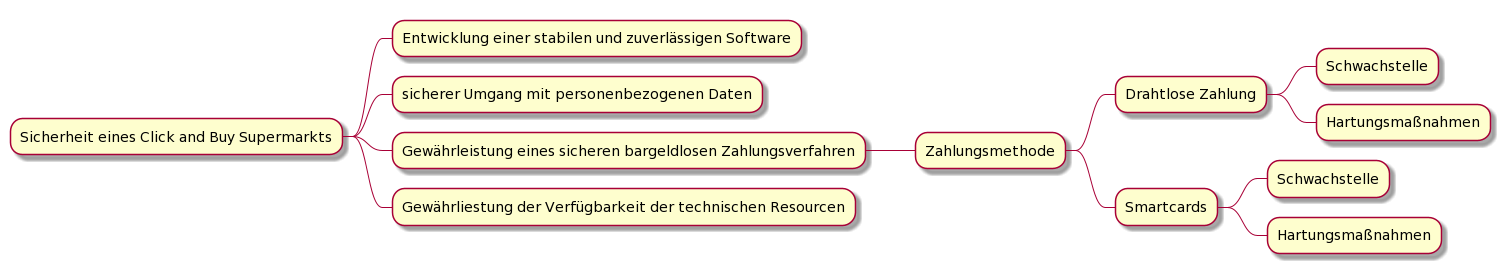
\includegraphics[width=20cm]{Bilder/Diagram2.png}}
         \caption{Recherchespfad\\ Quelle: eigene Darstellung}
          \label{fig:diagramfrage}
  \end{figure}
\end{landscape}


\subsection{Durchführung von Experimenten}
\textbf{Hier testen wir NFC und Smartcard vllt ohne und mit Hartungsmassnahmen, um zu zeigen, dass Massnahmen X gegen
Angriff Y geschützt ist}

Die Tests für die Objekte dieser Untersuchung sollen im Labor der Hochschule Worms durchgeführt werden. 
Dazu werden 3 Maschinen verwendet, die folgende Rollen übernahmen sollen: Server, Host und Angreifer. 
Der Host soll eine Anfrage an den Server schicken, die eine Simulation von einem Bezahlvorgang darstellen soll.
Der Server soll unter normalen Umstände auf diese Anfrage antworten und unter einem Angriff keine Antwort
geben. Dieses Verfahren findet sowohl bei Drahtlosen Verbindungen als auch bei Smartcards statt.


\subsubsection{Angriff und Härtungsmaßnahme einer drahtlosen Server}
Für dieses Experiment sollen folgende Angriffstechniken verwendet werden: \textit{Denial-of-Service}.

Im erstem Experiment wird der Host eine normale Anfrage an den Server schicken. Dieser wird standarmäßig konfiguriert,
also ohne irgendwelche Sicherheitsmechanismen, wie Authentifizierung, Überprüfung der Anzahl von Verbindungen oder Anfragen
nach Zertifikaten.

Der erste Angriff wird mithilfe des Tools \acrfull{nmap}\footnote{\acrshort{nmap} ist eine freie und Open Source Anwendung
für die Entdeckung und Sicherheitsüberprüfung von Netzwerken \cite{refst:nmap}.} durchgeführt werden. In diesem Angriff benutzt
der Angreifer eine weitere Maschine, um sich selbst zu verbergen und um den Angriff zu verstärken. Der Angreifer schickt extrem viele
Pakete\footnote{Pakete sind im Netzwerk die Einkapselung von Metainformationen, wie Quell- und Zieladresse Protokolltyp 
und Größe die Nutzdaten, wie Text, Videos oder Bilder \cite{refbook:SWIS}.} in sehr kürzem Abstand, um die Ressourcen des 
Servers komplett auszunutzen, sodass er auf keine Anfragen mehr antworten kann \cite{refip:KSDD}. 
Im folgenden gibt es eine Abbildung zu dieser Angriffstechnik:

\begin{figure}[H]
  \centering{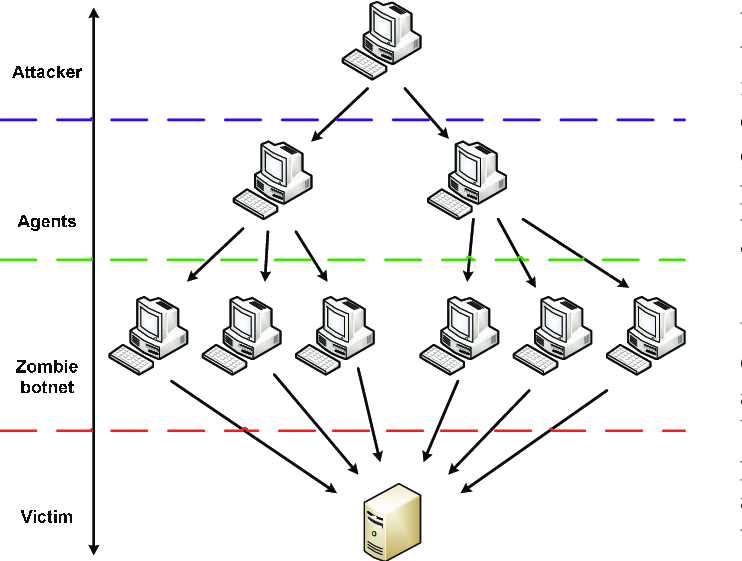
\includegraphics[width=8cm]{Bilder/refip_VDSD.png}}
  \caption{\acrfull{dos}\\ Quelle: Durcekova et al., 2012}
  \label{fig:VDSD}
\end{figure}
%\cite{refip:VDSD}

\subsubsection{Angriff und Härtungsmaßnahme von Smartcard}
\textbf{Ich würde nur das Beispiel von NFC geben und die anderen nur nach Bedarf hinzufügen, sonst werden wir hier
viele Seite haben}


\subsection{Beobachtung von Angriffsmöglichkeiten}
\textbf{Hier können wir sagen, dass wir in einem Labor einige Angriffe durchgeführt haben. Wir beschreiben alle Elementen
dieses Labor und was wir von diesem Experimenten erwarten. Auch die Quelle für solche Beobachtung.}

Bevor des Angriffes konnte der Host sich normal mit dem Server kommunizieren und Anfrage schicken und Antwort bekommen.
Während des Angriffes war die Kommunikation mit dem Server entweder zu langsam oder sogar unterbrochen. In diesem Fall
konnte konnte der Host selten Antwort auf Anfrage bekommen. In einigen Momenten gab es überhaubt keine Antwort. 

Von seits des Servers wurde das Tool Wireshark\footnote{Wireshark ist eine Anwendung für die Analyse von Networkprotoklle.
Es beschreibt ein- und ausgehende Pakete und dessen Bestandteile \cite{refst:wisa}.} verwendet, um die Ein- und Ausgehende
Pakete zu beobachten und zu analysieren \cite{refart:UBEC}. Unter normalen Umstände kamen die Pakete mit einem angemessen
Zeitabstand. Während des Angriffes bekem der Server viele kleine Pakete ohne nützlichen Inhalt und in sehr kürzem Zeitabstand.
Unter gibt es eine Abbildung, wie das Wireshark die Kommunikation aufzeichnet:

\begin{figure}[H]
  \centering{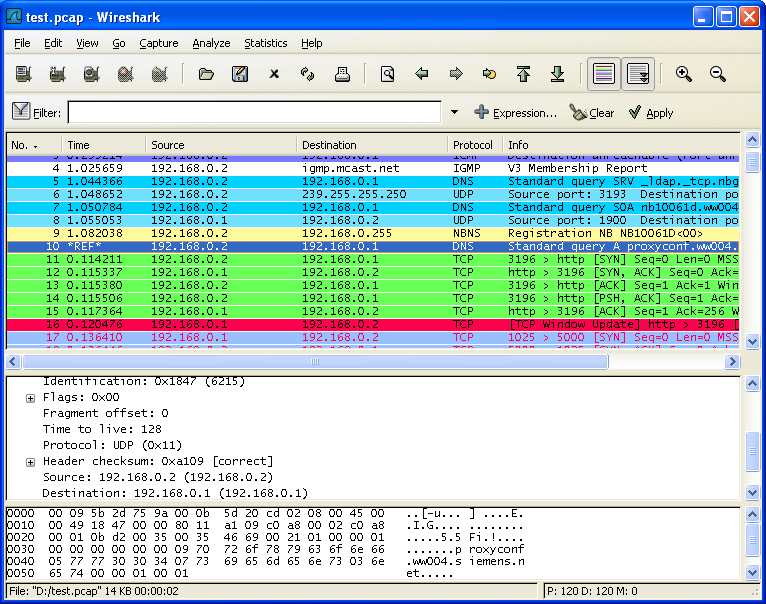
\includegraphics[width=8cm]{Bilder/refst_wisa.png}}
  \caption{Ausgabe von Wireshark \\Quelle: Wireshark, 2021}
  \label{fig:refst_wisa}
\end{figure}
%\cite{refst:wisa}

Wie \cite{refip:NYRS} vorschlug, um den Angriff zu verhindern wurde der Server erneut konfigurieren, indem er nur
Kommunikation von registrierten Hosts zu akzeptierte. Nach dieser Anpassung war der Angreifer nicht mehr in der Lage, 
sich mit dem Server zu verbinden, da er keine registrierte Nutzer war. Aus der Aufzeichnung von Wireshark wurden nicht 
angemeldete Pakete direkt verworfen.

\subsection{Interview mit IT-SicherheitsFirmen}

\textbf{Hier schreiben wir, dass wir Person x der Firma y nach dem ihrem Produkt bezüglich auf Sicherheit gefragt haben.
Vllt. 9 Frage, 3 über das Produkt, 3 über Schwachstelle und 3 über Härtung. Wir brauchen auch am Anfang irgendwelche Zitation
wie eine wissenschaftliche Interview aussehen sollte.}

\subsection{Literaturrecherche}

Die Literatur bezüglich Netzwerksicherheit, bargeldlose Zahlungsverfahren und Vending Machines ist in den 
letzten 20 Jahren deutlich umfangreicher geworden. Da diese Begriffe viele und fast unendliche Konzepte 
decken, gehen wir hier auf spezifische Aspekte dieser Begriffe ein und zwar auf die Sicherheit von drahtlosen 
Zahlungsmethode und von Smartcards. 

Folgende Quelle trugen zu der Suchen nach vertrauenswürdigen Literaturquelle bei:

\begin{itemize}
    \item ScienceDirect
    \item Researchg Gate
    \item IEEE Xplore
    \item Google Scholar.
\end{itemize}

Diese Quellen ermöglichten ein allgemeines theoretisches Kenntnis über das Objekt dieser Untersuchung und dessen aktuellen 
Stand der Entwicklung.
